\documentclass[12pt]{article}
\usepackage{amsmath,amsthm,amssymb,MnSymbol,enumerate,fullpage,graphicx}
\setlength{\parindent}{0in}

\title{PGM 10-708: HW 2}
\author{Willie Neiswanger\\
\texttt{willie@cs.cmu.edu}}
\date{}

\begin{document}

\maketitle


\section*{Problem 1}
\label{sec:prob1}

\subsection*{1.1}
Let $\textbf{x} = (x_1,\ldots,x_p) \sim p(\textbf{x} | 0, \Sigma) = \text{Normal}(0,\Sigma)$, and $\Omega = \Sigma^{-1}$.

\subsubsection*{1.1.a}
Let $\textbf{x} = (\textbf{x}_1,\textbf{x}_2)$, where $\textbf{x}_1$ and $\textbf{x}_2$ form a partition of the $p$ variables, and 
$(\textbf{x}_1,\textbf{x}_2) \sim 
\text{Normal} \left( \left[ \begin{smallmatrix} \textbf{x}_1 \\ \textbf{x}_2 \end{smallmatrix} \right] | 0, \left[ \begin{smallmatrix} \Sigma_{1,1}& \Sigma_{1,2} \\ \Sigma_{2,1} & \Sigma_{2,2} \end{smallmatrix} \right] \right)$.
Derive $p(\textbf{x}_1 | \textbf{x}_2)$.\\

Denote the block precision matrix as 
$ \left[ \begin{smallmatrix} \Omega_{1,1}& \Omega_{1,2} \\ \Omega_{2,1} & \Omega_{2,2} \end{smallmatrix} \right] = 
\left[ \begin{smallmatrix} \Sigma_{1,1}& \Sigma_{1,2} \\ \Sigma_{2,1} & \Sigma_{2,2} \end{smallmatrix} \right]^{-1} $.
Consider the quadratic form of the exponent of 
$\text{Normal} \left( \left[ \begin{smallmatrix} \textbf{x}_1 \\ \textbf{x}_2 \end{smallmatrix} \right] | 0, \left[ \begin{smallmatrix} \Sigma_{1,1}& \Sigma_{1,2} \\ \Sigma_{2,1} & \Sigma_{2,2} \end{smallmatrix} \right] \right)$
i.e., $-\frac{1}{2} \textbf{x}^{\top} \Sigma^{-1} \textbf{x} = 
-\frac{1}{2} \textbf{x}_1^{\top} \Omega_{11} \textbf{x}_1 
-\frac{1}{2} \textbf{x}_1^{\top} \Omega_{12} \textbf{x}_2   
-\frac{1}{2} \textbf{x}_2^{\top} \Omega_{21} \textbf{x}_1 
-\frac{1}{2} \textbf{x}_2^{\top} \Omega_{22} \textbf{x}_2
$. As this is still a quadratic form, we know that $p(\textbf{x}_1 | \textbf{x}_2)$ is still a Gaussian. The goal is now to find the mean and covariance of this distribution.
%Note that the quadratic form of the original exponent can be written
%$-\frac{1}{2} \textbf{x}^{\top} \Sigma^{-1} \textbf{x} = 
By inspecting the above equality, we can pick out the first term 
$-\frac{1}{2} \textbf{x}_1^{\top} \Omega_{11} \textbf{x}_1$. Regarding $\textbf{x}_1$ as our observation and $\textbf{x}_2$ as a constant, this has the same form of our original Gaussian, 
and implies that the covariance for the conditional distribution 
\begin{equation}
    \Sigma_{1|2} = \Omega_{11}^{-1}.
\end{equation}
Through inspection we see that the terms linear in $\textbf{x}_1$ are 
$\textbf{x}_1^{\top}[\Omega_{12}\textbf{x}_2]$ (where we've used the fact that $\Omega_{21}^{\top} = \Omega_{12}$).
This implies that the coefficient of $\textbf{x}_1$ in this expression must equal $\Sigma_{1|2}^{-1} \mu_{1|2}$, and hence
\begin{equation}
    \mu_{1|2} = \Sigma_{1|2}[\Omega_{12}\textbf{x}_2] = - \Omega_{11}^{-1} \Omega_{12} \textbf{x}_2
\end{equation}
In order to write $\Sigma_{1|2}$ and $\mu_{1|2}$ in terms of the original parameter $\Sigma$, we use the Schur complement of the matrix, using the definition
$\left[ \begin{smallmatrix} \Sigma_{1,1}& \Sigma_{1,2} \\ \Sigma_{2,1} & \Sigma_{2,2} \end{smallmatrix} \right]^{-1} = 
 \left[ \begin{smallmatrix} \Omega_{1,1}& \Omega_{1,2} \\ \Omega_{2,1} & \Omega_{2,2} \end{smallmatrix} \right]$,
 we have the relation
 \begin{equation}
    \begin{split}
        \Omega_{11} &= (\Sigma_{11} - \Sigma_{12} \Sigma_{22}^{-1} \Sigma_{21})\\
        \Omega_{12} &= - (\Sigma_{11} - \Sigma_{12} \Sigma_{22}^{-1} \Sigma_{21})^{-1} \Sigma_{12} \Sigma_{22}^{-1}
    \end{split}
\end{equation}
We substitute these in the expressions above for $\Sigma_{1|2}$ and $\mu_{1|2}$ to get
\begin{equation}
    \begin{split}
        \mu_{1|2} &= \Sigma_{12} \Sigma_{22}^{-1} \textbf{x}_2 \\
        \Sigma_{1|2} &=  \Sigma_{11} - \Sigma_{12} \Sigma_{22}^{-1} \Sigma_{21}
    \end{split}
\end{equation}


\subsubsection*{1.1.b}
We can write the precision matrix in block form as $\Omega = \left[ 
\begin{smallmatrix} \Omega_{1,1} & \Omega_{1,2} \\ \Omega_{2,1} & \Omega_{2,2}
\end{smallmatrix} \right]$.
Derive $\text{Var}(\textbf{x}_1 | \textbf{x}_2)$ in terms of $\Omega$.\\

Using part of the derivation from (1.1.a), we know that $\textbf{x}_1 | \textbf{x}_2$ is normally distributed, and that the variance in terms of $\Omega$ can be written
\begin{equation}
    \Sigma_{1|2} = \Omega_{11}^{-1}.
\end{equation}


\subsubsection*{1.1.c}
Argue that $\Omega_{i,j}=0$ iff $x_i \upmodels x_j | \text{rest}$.\\

Let $\textbf{x}_1 = (x_i,x_j)$ and $\textbf{x}_2 = \textbf{x}_{-(i,j)}$ (i.e. $\textbf{x}_2$ is all other $x_i$'s).
%Then, if $\Omega_{i,j} = 0$, 
From part $1.1.a$ we know that $P((x_i,x_j) | \textbf{x}_2)$ is Gaussian with covariance matrix $\Omega_{11}^{-1}$, recalling that we've defined $\Sigma = \left[ \begin{smallmatrix} \Omega_{1,1}& \Omega_{1,2} \\ \Omega_{2,1} & \Omega_{2,2} \end{smallmatrix} \right]^{-1}$. Therefore, if $\Omega_{ij} = \Omega_{ji} = 0$, then $\Omega_{11}^{-1}$ is symmetric. Since $P((x_i,x_j) | \textbf{x}_2)$ is Gaussian distributed with a symmetric covariance matrix, we know that $x_i \upmodels x_j | \textbf{x}_2$. \\

On the other hand, if $x_i \upmodels x_j | \textbf{x}_2$, then the covariance matrix of the Gaussian $P((x_i,x_j) | \textbf{x}_2)$ is diagonal, and so $\Omega_{ij} = \Omega_{ji} = 0$.


\subsection*{1.2}
Let $\textbf{x}_1, \ldots, \textbf{x}_n$ $\sim$ $\text{Normal}(0,\Sigma)$, where $\textbf{x}_i = (x_i^1, \ldots x_i^p)$. Let $\Theta = \Sigma^{-1}$ and $S = \sum_i \frac{\textbf{x}_i \textbf{x}_i^\top}{n}$. Show that the log-likelihood of the multivariate Normal distribution to to be optimized is equal to $\text{log} \text{ det} \Theta - \text{tr}(S\Theta)$.\\

This holds because 
\begin{equation}
    \begin{split}
        \text{log} \left( \prod_i \text{Normal}(\textbf{x}_i | 0,\Theta^{-1}) \right) 
        &= -\frac{np}{2}\text{log}(2\pi) - \frac{n}{2} \text{log} \text{ det}(\Theta^{-1}) - \frac{1}{2} \sum_i \textbf{x}_i^{\top} \Theta \textbf{x}_i\\
        &= -\frac{np}{2}\text{log}(2\pi) + \frac{n}{2} \text{log} \text{ det}(\Theta) - \frac{1}{2} \sum_i \textbf{x}_i^{\top} \Theta \textbf{x}_i
    \end{split}
\end{equation}
Considering only terms that include the parameter and disregarding coefficients, we can see that optimizing the above expression is therefore equivalent to (i.e. can be achieved by) optimizing $\text{log} \text{ det}(\Theta) - \text{tr}(S\Theta)$.


\subsection*{1.3}
Implement the Meinshausen-Buhlmann and Glasso algorithms.\\

The estimated precision matrices are drawn below (where white elements in the adjacency matrix imply edges and black implies no edges). It seems that the estimated precision matrices become more sparse as the lambda parameter is increased.
\begin{figure}[h!]
    \centering
    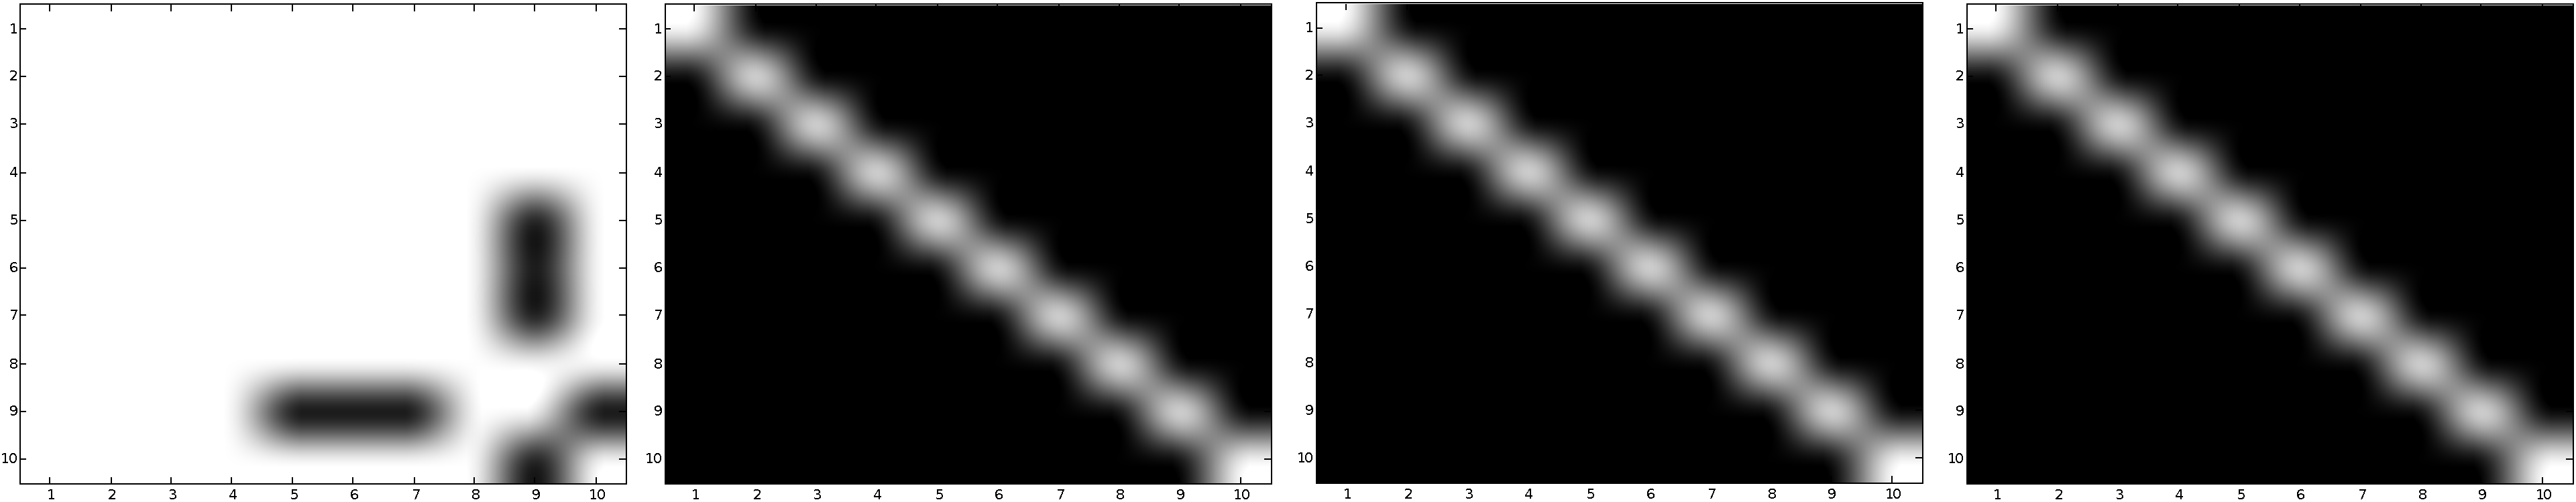
\includegraphics[width=0.9\textwidth]{precImg/mbPrec.pdf}
    \caption{MB algorithm results for $\lambda = [0,20,30,40]$.}
\end{figure}
\begin{figure}[h!]
    \centering
    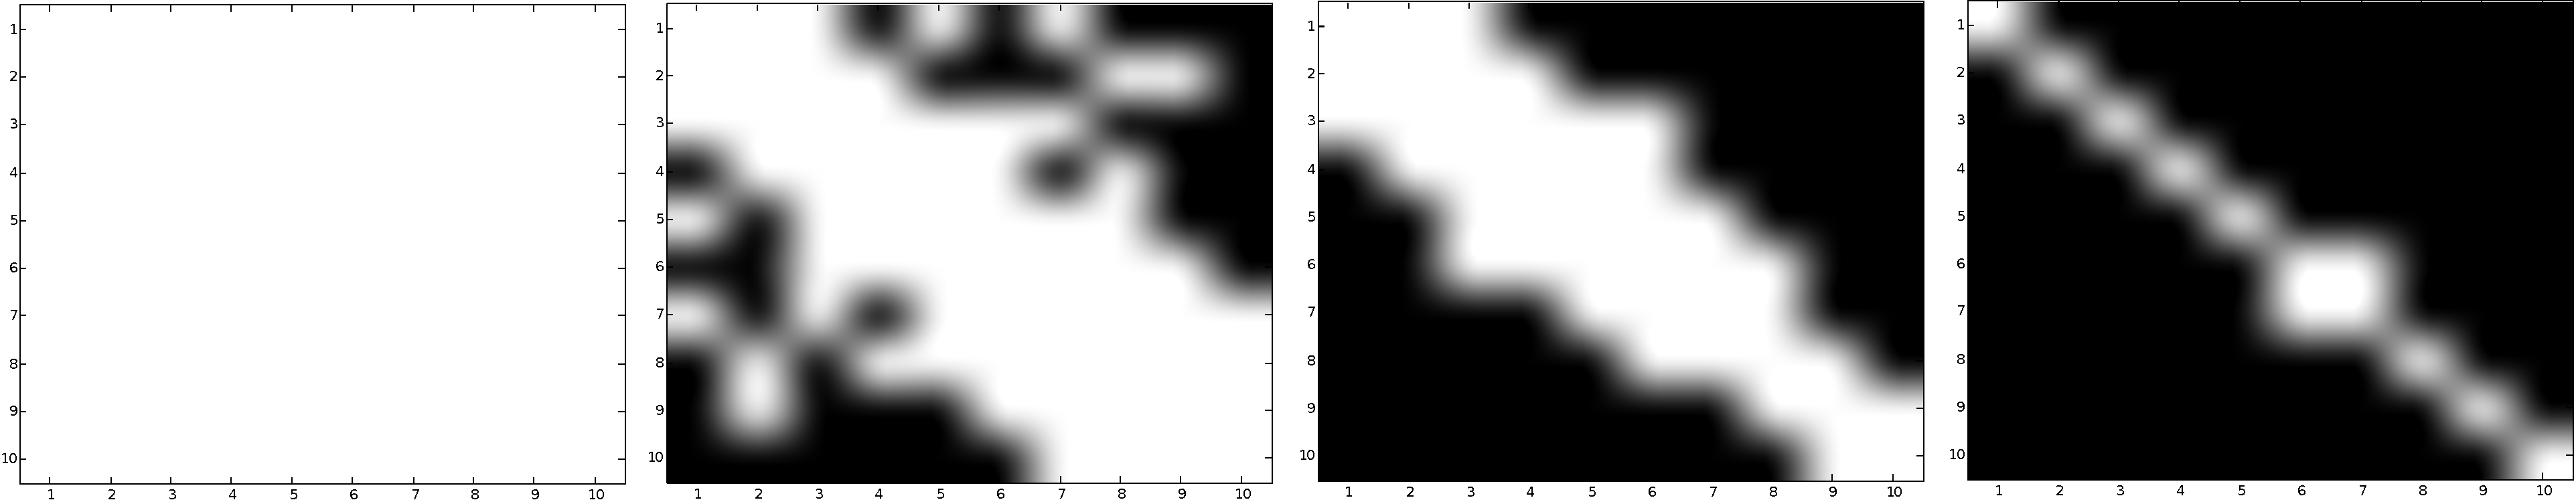
\includegraphics[width=0.9\textwidth]{precImg/glPrec.pdf}
    \caption{Glasso algorithm results for $\lambda = [0,0.2,0.5,0.8]$.}
\end{figure}



\section*{Problem 2}
\label{sec:prob2}
Assume, for simplicity, that we denote $P(z_1) = P(z_1 | z_0) = \eta_{z_0,z_1}$

\subsection*{2.1}
The parameters of this model are $\theta$ (dimension $K$), $\sigma^2$ (dimension $K$), $\eta$ (a matrix of size $K \times K$), and $\gamma$ (dimension $K$).

\subsection*{2.2}
%Write the expected conditional log-likelihood for data $(x_1,y_1),\ldots,(x_n,y_n)$.
%\\

The conditional log-likelihood can be written and lower bounded by the following:
\begin{equation*}
    \begin{split}
        &\text{log}(P(\textbf{Y} | \textbf{X})) = \text{log} \left( \sum_{\textbf{Z}} P(\textbf{Y},\textbf{Z} | \textbf{X}) \right)
             = \text{log} \left( \sum_{\textbf{Z}} P(\textbf{Z} | \textbf{X}) P(\textbf{Y} | \textbf{Z}, \textbf{X}) \right)\\
        & =  \text{log} \left( \mathbb{E}_q \left[ P(\textbf{Z} | \textbf{X}) P(\textbf{Y} | \textbf{Z}, \textbf{X}) \frac{1}{q(\textbf{Z})} \right] \right)
             \text{ \hspace{3mm}(for a distribution $q$ over $Z$)}\\
        & \geq  \mathbb{E}_q \left[  \text{log} \left( P(\textbf{Z} | \textbf{X}) P(\textbf{Y} | \textbf{Z}, \textbf{X}) 
            \frac{1}{q(\textbf{Z})} \right) \right]
             \text{ \hspace{3mm}(using Jensen's inequality)}\\
        & = \mathbb{E}_q \left[ \text{log} \left( P(\textbf{Z} | \textbf{X}) \right) \right] 
             + \mathbb{E}_q \left[\text{log} \left( P(\textbf{Y} | \textbf{Z}, \textbf{X}) \right) \right] 
             - \mathbb{E}_q \left[\text{log} \left( q(\textbf{Z}) \right) \right] \\
        & = \mathbb{E}_q \left[ \sum_i \text{log} \left( P(z_i | z_{i-1}, x_i) \right)
             + \sum_i \text{log} \left( P(y_i | z_i, x_i) \right) \right] 
             - \mathbb{E}_q \left[\text{log} \left( q(\textbf{Z}) \right) \right] \\
        & = \mathbb{E}_q \left[ \sum_i (\text{log}(\eta_{z_{i-1},z_i}) + \gamma_{z_i}^{\top} x_i )
             + \sum_i \text{log} \left( \text{Normal}(y_i | \theta_{z_i}^{\top} x_i, \sigma_{z_i}^2) \right) \right] 
             - \mathbb{E}_q \left[\text{log} \left( q(\textbf{Z}) \right) \right] \\
        & = \mathbb{E}_q \left[ \sum_i \left( \text{log}(\eta_{z_{i-1},z_i}) + \gamma_{z_i}^{\top} x_i 
             -\frac{1}{2}\left( \text{log}(2\pi) - \text{log}(\sigma_{z_i}^2) - \frac{(y_i - \theta_{z_i}^{\top} x_i)^2}{ \sigma_{z_i}^2} \right)  \right) \right]
             - \mathbb{E}_q \left[\text{log} \left( q(\textbf{Z}) \right) \right] \\
         %& =  \sum_i \sum_{z_i} \sum_{z_{i-1}} \left( \text{log}(\eta_{z_{i-1},z_i}) + \gamma_{z_i}^{\top} x_i 
             %-\frac{1}{2}\left( \text{log}(2\pi) - \text{log}(\sigma_{z_i}^2) - \frac{(y_i | \theta_{z_i}^{\top} x_i)^2}{ \sigma_{z_i}^2} \right)  \right)
             %- \mathbb{E}_q \left[\text{log} \left( q(\textbf{Z}) \right) \right] \\
        %%
        %
        %
        %& = \sum_i \left( \mathbb{E}_q\left[ \text{log}(\eta_{z_{i-1},z_i}) \right] + \mathbb{E}_q\left[ \gamma_{z_i}^{\top} x_i \right]
             %-\frac{1}{2}\left( \text{log}(2\pi) - \mathbb{E}_q\left[ \text{log}(\sigma_{z_i}^2) \right] - 
                %\mathbb{E}_q\left[ \frac{(y_i | \theta_{z_i}^{\top} x_i)^2}{ \sigma_{z_i}^2} \right] \right)  \right)
             %- \mathbb{E}_q \left[\text{log} \left( q(\textbf{Z}) \right) \right] \\
        %
        %
        %& = \text{log} \left( \prod_{i=1}^p \sum_{z_i}  e^{\gamma_{z_i}^{\top} x_i} \eta_{z_{i-1},z_i} 
            %\text{Normal}(y_i | \theta_{z_i}^{\top} x_i, \sigma_{z_i}^2) \right)\\
        %& = \sum_{i=1}^p \text{log} \left( \sum_z e^{\gamma_{z_i}^{\top} x_i} \eta_{z_{i-1},z_i} 
            %\text{Normal}(y_i | \theta_{z_i}^{\top} x_i, \sigma_{z_i}^2) \right)\\
        %&\sum_{i=2}^p \left( \gamma_{z_i}^{\top} x_i + \text{log}(\eta_{z_{i-1},z_i}) + 
            %\text{log}(\text{Normal}(y_i | \theta_{z_i}^{\top} x_i, \sigma_{z_i}^2)) \right)
    \end{split}
\end{equation*}
This is the EM objective function; note that the second element of the final term is the entropy.\\
%Therefore, the expected conditional log-likelihood is 
%\begin{equation}
    %\begin{split}
        %&\mathbb{E} \left[ \text{log} (P(\textbf{Y} | \textbf{X})) \right]
            %= \sum_{i=1}^p \mathbb{E} \left[ \text{log} \left( \sum_z e^{\gamma_{z_i}^{\top} x_i} \eta_{z_{i-1},z_i} 
            %\text{Normal}(y_i | \theta_{z_i}^{\top} x_i, \sigma_{z_i}^2) \right) \right] \\
        %&\mathbb{E} \left[ \text{log} (P(\textbf{Y} | \textbf{X})) \right]
    %\end{split}
%\end{equation}
%Using Jensen's inequality we can provide a lower bound to the above quantity with 
%\begin{equation}
    %\begin{split}
        %&\mathbb{E} \left[ \text{log} (P(\textbf{Y} | \textbf{X})) \right] \leq 2\\
        %&\mathbb{E} \left[ \text{log} (P(\textbf{Y} | \textbf{X})) \right] \leq 2
    %\end{split}
%\end{equation}

\subsection*{2.3}
Derive the update equations for the EM algorithm for this model.
\\

We first write the EM objective as
\begin{equation}
    \begin{split}
        &= \mathbb{E}_q \left[ \sum_i \left( \text{log}(\eta_{z_{i-1},z_i}) + \gamma_{z_i}^{\top} x_i 
             -\frac{1}{2}\left( \text{log}(2\pi) - \text{log}(\sigma_{z_i}^2) - \frac{(y_i - \theta_{z_i}^{\top} x_i)^2}{ \sigma_{z_i}^2} \right)  \right) \right]
             - \mathbb{E}_q \left[\text{log} \left( q(\textbf{Z}) \right) \right] \\
         &=  \sum_i \sum_{z_i} \sum_{z_{i-1}} \left( \text{log}(\eta_{z_{i-1},z_i}) + \gamma_{z_i}^{\top} x_i 
             -\frac{1}{2}\left( \text{log}(2\pi) - \text{log}(\sigma_{z_i}^2) - \frac{(y_i - \theta_{z_i}^{\top} x_i)^2}{ \sigma_{z_i}^2} \right)  \right)
             - \mathbb{E}_q \left[\text{log} \left( q(\textbf{Z}) \right) \right] \\
    \end{split}
\end{equation}

Let the EM object function above be written $\mathcal{L}(\theta,q)$, where $\theta$ are the model parameters and $q$ is the distribution over $\textbf{Z}$. For a version of EM, we can formulate the E-step as updating the distribution $q$ in the following way: 
\begin{equation}
    \begin{split}
        & q^{(t+1)} = \text{argmax}_q \mathcal{L}(q,\theta^{(t)}) = P(\textbf{Z} | \textbf{Y}, \textbf{X}, \theta^{(t)})
            = \frac{1}{K} P(\textbf{Y} | \textbf{Z}, \textbf{X}, \theta^{(t)}) P(\textbf{Z} | \textbf{X}, \theta^{(t)}) \\
        & = \frac{1}{K} \prod_i P(y_i | x_i, z_i) \prod_i P(z_i | x_i, z_{i-1})
            = \frac{1}{K} \prod_i \text{Normal}(y_i | \theta_{z_i}^{\top} x_i, \sigma_{z_i}^2)  
            \eta_{z_{i-1},z_i} e^{\gamma_{z_i}^{\top} x_i}
    \end{split}
\end{equation}
where in this case the normalizing constant $K$ is computed by summing over the latent variables $\textbf{Z}$ in the numerator.
\\

And we can write the M-step as:
\begin{equation}
    \theta^{(t)} = \text{argmax}_{\theta} \mathcal{L}(q^{(t+1)},\theta)
\end{equation}
This involves maximizing the objective function 
\begin{equation}
    \begin{split}
        & 2\sum_i \sum_{z_i} \sum_{z_{i-1}} \left( \text{log}(\eta_{z_{i-1},z_i}) + \gamma_{z_i}^{\top} x_i 
             -\frac{1}{2}\left( \text{log}(2\pi) - \text{log}(\sigma_{z_i}^2) - \frac{(y_i | \theta_{z_i}^{\top} x_i)^2}{ \sigma_{z_i}^2} \right)  \right)
    \end{split}
\end{equation}
with respect to the parameters $\eta_{z_{i-1},z_i}$, $\gamma_{z_i}$, $\theta_{z_i}$, and $\sigma_{z_i}^2$.
By taking the gradient of the EM objective function with respect to each parameter, setting it to zero, and solving.
Solving for each gradient is omitted due to time constraints $\ddot\frown$.


\section*{Problem 3}
\label{sec:prob3}
The KL divergence can be written 
\begin{equation}
    \begin{split}
        &\text{KL}(P(x|\theta),P(x|\eta)) = \int_x \log\left(\frac{P(x|\theta)}{P(x|\eta)}\right)P(x|\theta) 
            = \int_x \left( \text{log}P(x|\theta) - \text{log}P(x|\eta) \right) P(x|\theta) \\
        & = \int_x P(x|\theta) \text{log}P(x|\theta) - \int_x P(x|\theta) \text{log}P(x|\eta) \\
        & = \int_x P(x|\theta) \left( \sum_{i=1}^k \theta_i f_i(x) - A(\theta)  \right) -   
                \int_x P(x|\theta) \left( \sum_{i=1}^k \eta_i f_i(x) - A(\eta)  \right) \\
        & = \int_x P(x|\theta) \sum_{i=1}^k \theta_i f_i(x) - \int_x P(x|\theta) A(\theta)  -   
                \int_x P(x|\theta) \sum_{i=1}^k \eta_i f_i(x) - \int_x P(x|\theta) A(\eta) \\
        & = \int_x P(x|\theta) \sum_{i=1}^k \theta_i f_i(x) - \int_x P(x|\theta) \sum_{i=1}^k \eta_i f_i(x) 
            - A(\theta) + A(\eta)\\
        & = \int_x P(x|\theta) \left( \sum_{i=1}^k (\theta_i - \eta_i) f_i(x) \right)- A(\theta) + A(\eta)\\
        & = \sum_{i=1}^k (\theta_i - \eta_i) \int_x P(x|\theta) f_i(x) - A(\theta) + A(\eta)\\
        & = \sum_{i=1}^K (\theta_i - \eta_i) \frac{\partial A(\theta)}{\partial \theta_i} - A(\theta) + A(\eta)
    \end{split}
\end{equation}
To show the last equality holds, we need to show that $\int_x P(x|\theta) f_i(x) = \frac{\partial A(\theta)}{\partial \theta_i}$. This holds because $P(X|\theta) = \frac{\text{exp}(\sum_i \theta_i f_i(x))}{\text{exp}(A(\theta))}$, hence due to normalization $A(\theta) = \text{log}\int_x \text{exp}(\sum_i \theta_i f_i(x))$.
Therefore,
\begin{equation}
    \begin{split}
        \frac{\partial A(\theta)}{\partial \theta_j}
            &= \frac{1}{\int_x \text{exp}(\sum_i \theta_i f_i(x))}   \int_x \text{exp}(\sum_i \theta_i f_i(x)) f_j(x) \\
            &= \frac{1}{\text{exp}(A(\theta))} \int_x \text{exp}(\sum_i \theta_i f_i(x)) f_j(x) 
                = \int_x \text{exp}(\sum_i \theta_i f_i(x) - A(\theta)) f_j(x) \\
            &= \int_x P(X|\theta)f_j(x)
    \end{split}
\end{equation}
Hence $\int_x P(x|\theta) f_i(x) = \frac{\partial A(\theta)}{\partial \theta_i}$ and this completes the proof.


\section*{Problem 4}
\label{sec:prob4}

The IPF update rule is: $\Psi_C(x_C)^{(t+1)} = \Psi_C(x_C)^{(t)} \frac{\tilde{p}(x_C)}{p^{(t)}(x_C)}$.\\

We can write
\begin{equation}
    \begin{split}
        p^{(t+1)}(x_U) 
            &= \frac{1}{Z} \prod_D \psi_D(x_D)^{(t+1)}
                = \frac{1}{Z} \left( \prod_{D \neq C} \psi_D(x_D)^{(t+1)} \right) \psi_C(x_C)^{(t+1)}\\
            &= \frac{1}{Z} \left( \prod_{D \neq C} \psi_D(x_D)^{(t+1)} \right) 
                \psi_C(x_C)^{(t)} \frac{\tilde{p}(x_C)}{p^{(t)}(x_C)}  \hspace{3mm} 
                \text{(using the update rule)} \\
            &= \frac{1}{Z} \left( \prod_{D} \psi_D(x_D)^{(t)} \right) 
                \frac{\tilde{p}(x_C)}{p^{(t)}(x_C)} 
                = \frac{1}{Z} p^{(t)}(x_U) \frac{\tilde{p}(x_C)}{p^{(t)}(x_C)} \\
            &= p^{(t)}(x_{U \setminus C} | x_C) \tilde{p}(x_C)
    \end{split}
\end{equation}
where the third to last equality holds as we only use the update for the $C^{th}$ $\psi$, so 
$\prod_{D \neq C} \psi_D(x_D)^{(t+1)} = \prod_{D \neq C} \psi_D(x_D)^{(t)}$.


\end{document}
